\chapter{2D case}

% {{{1 PROBLEM
\section{Problem}

In this part, we will focus on a 2D point cloud and we will use for the energy
the area of the $ r $-offset of a point cloud $ X $: the Minkowski sum with an
euclidean ball $ B(0, r) $.

We will also choose other types of energies like the perimeter of the boundary,
the weighted area (the gradient of a Voronoi cell is weighted by its
corresponding area) and the weighted perimeter.

Firstly, we will show how to compute the area of the union of balls or more
generally any quantity computed on the intersection of a Voronoi cell and a
circle. Then, we will run different experiments to verify that the gradient of
the union of balls is proportional to the mean curvature of the underlying
hypersurface. Finally, we will run our programs on different point clouds with
different parameters to show that it can simulate discrete mean curvature flows.

% {{{1 AREA OF A UNION OF BALLS
\section{Area of a union of balls}

In order to compute this energy, we need to know how to estimate the area of the
intersection of a ball and a Voronoi cell. Indeed, the area of the union of
balls is the same as the sum of the areas of the restrictions of the balls to
their Voronoi cell (because the Voronoi cells partition the plane).

This is the same work as the one done in \cite{cazals2011computing} except that
we restrict ourselves to 2D which is simpler than in 3D.

For doing that, we need to decompose the intersection into triangles and
spherical caps.

\ref{fig:inter_voronoi_ball_2d} illustrates the different cases for the
intersection of a Voronoi cell and a ball in 2D.

\begin{figure}[h]
    \centering
    \begin{minipage}{0.32\linewidth}
        \centering
        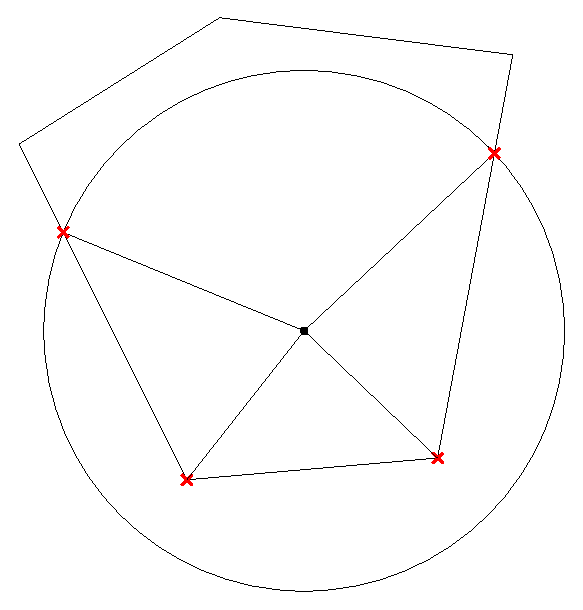
\includegraphics[scale=0.4]{2d/inter_voronoi_ball_2d}
        \subcaption{General case}
        \label{fig:inter_voronoi_ball_2d:a}
    \end{minipage}
    \begin{minipage}{0.32\linewidth}
        \centering
        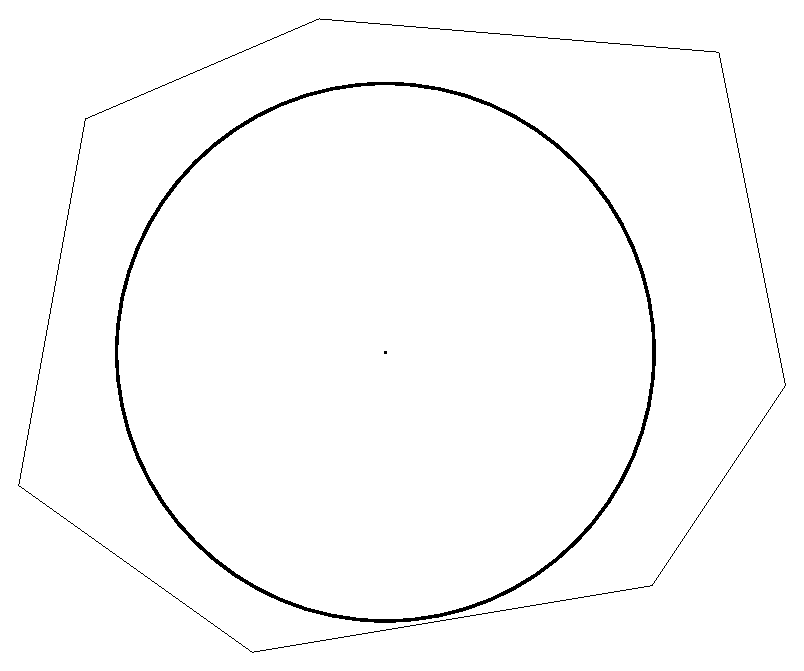
\includegraphics[scale=0.4]{2d/inter_voronoi_ball_2d_no_inter}
        \subcaption{No intersections}
        \label{fig:inter_voronoi_ball_2d:b}
    \end{minipage}
    \begin{minipage}{0.32\linewidth}
        \centering
        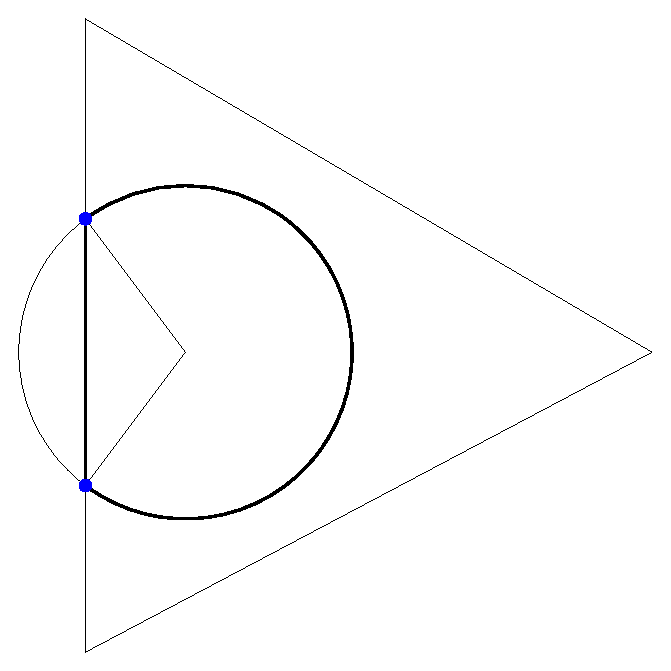
\includegraphics[scale=0.4]{2d/inter_voronoi_ball_2d_2_inter}
        \subcaption{2 intersections}
        \label{fig:inter_voronoi_ball_2d:c}
    \end{minipage}

   \caption{Different cases for the intersection between a Voronoi cell and a sphere}
   \label{fig:inter_voronoi_ball_2d}
\end{figure}

We used \texttt{CGAL} to compute the Delaunay triangulation of our point set.
Given this triangulation, we can compute the Voronoi cell of a point by doing
the following:
\begin{enumerate}
    \item Access the neighbouring faces of a vertex using the
        \texttt{incident\_faces} method.
    \item Compute the Voronoi vertices of these faces using the \texttt{dual}
        method.
\end{enumerate}

Then, we will need to know the vertices of the boundary of the intersection (the
points forming the bold boundary in \ref{fig:inter_voronoi_ball_2d}). There are
two types of those points: some are Voronoi vertices and some are intersections
of Voronoi edges and circles. To each of these points, we attach a boolean
saying whether the point is an interior point or an intersection one. We also
attach the corresponding Voronoi edge.

Then, we loop over the Voronoi edges $ e = pq $ of a vertex $ v $:
\begin{itemize}
    \item if $ p $ and $ q $ are interior points, we add the triangle $ pvq $.
    \item if $ p $ or $ q $ is interior point, we add the triangle $ pvq $.
    \item if $ p $ and $ q $ are intersection points, then if they belong to the
        same Voronoi edge, we add the triangle $ pvq $. If not, we add the
        angular sector $ \vec{vp}, \vec{vq} $.
\end{itemize}

Some special cases need to be handled:
\begin{itemize}
    \item the boundary of the Voronoi cell is entirely outside the ball, then we
        add $ \pi r^2 $ to the area of the union (see
        \ref{fig:inter_voronoi_ball_2d:b}).
    \item the boundary consists of two intersection points $ p $ and $ q $, then
        we add the triangle $ pvq $ and the angular sector $ \vec{vp}, \vec{vq}
        $ (see \ref{fig:inter_voronoi_ball_2d:c}).
    \item there is only one point on the boundary (can happen if adjacent balls
        are tangential), then we add $ \pi r^2 $.
\end{itemize}

We used the same techniques for computing the perimeter of the boundary of the
intersection except that if there are no intersection then the perimeter is null
and instead of adding triangles areas or angular sectors, we add lengths of
circular arcs.

% {{{1 IMPLEMENTATION DETAILS
\section{Implementation details}

For the implementation, we used different libraries: \texttt{CGAL} which is a
C++ library that offers all the basic geometric types (point, vector, line,
plane..), data structures and algorithms (triangulations...). We also used
\texttt{Eigen} which is a C++ linear algebra library which provides types such
as vector, matrix and manipulation operations. We used \texttt{Qt} for the GUI
programming.

The main difficulty here was to compute the intersection between a Voronoi cell
and a circle. The Voronoi cell is computed using its dual graph: the Delaunay
triangulation.

Then the automatic differentiation technique allowed us to only care about the
computation of the area and not its gradient.

% TODO

% {{{1 GRADIENT
\section{Gradient}

Then, we used the automatic differentiation technique described in
\ref{appendix:ad} to compute the gradient of the previously computed area.

See \ref{fig:gradients_area_2d} for a few examples of such gradients for different input point sets.

\begin{figure}[h]
    \centering

    \begin{minipage}{0.8\linewidth}
        \centering
        \includegraphics[scale=0.3]{2d/area/ellipse-100-01-15}
        \includegraphics[scale=0.3]{2d/area/ellipse-100-01-15-gradients}
        \subcaption{Gradients of the area for 100 samples on an ellipse}
        \label{fig:gradients_area_2d_ellipse}
    \end{minipage}

    \begin{minipage}{0.8\linewidth}
        \centering
        \includegraphics[scale=0.32]{2d/area/circle-100-01-15}
        \includegraphics[scale=0.32]{2d/area/circle-100-01-15-gradients}
        \subcaption{Gradients of the area for 100 samples on a circle}
        \label{fig:gradients_area_2d_circle}
    \end{minipage}

    \begin{minipage}{0.8\linewidth}
        \centering
        \includegraphics[scale=0.32]{2d/area/square-76-001-100}
        \includegraphics[scale=0.32]{2d/area/square-76-001-100-gradients}
        \subcaption{Gradients of the area for 100 samples on a square}
        \label{fig:gradients_area_2d_square}
    \end{minipage}

    \caption{Input point set / Computed gradients of the area}
    \label{fig:gradients_area_2d}
\end{figure}

We did the same thing using the gradient of the perimeter of the boundary on the
same point clouds (see \ref{fig:gradients_perimeter_2d}).

\begin{figure}[h]
    \centering

    \begin{minipage}{0.8\linewidth}
        \centering
        \includegraphics[scale=0.3]{2d/perimeter/ellipse-100-01-15}
        \includegraphics[scale=0.3]{2d/perimeter/ellipse-100-01-15-gradients}
        \subcaption{Gradients of the perimeter for 100 samples on an ellipse}
        \label{fig:gradients_perimeter_2d_ellipse}
    \end{minipage}

    \begin{minipage}{0.8\linewidth}
        \centering
        \includegraphics[scale=0.32]{2d/perimeter/circle-100-01-15}
        \includegraphics[scale=0.32]{2d/perimeter/circle-100-01-15-gradients}
        \subcaption{Gradients of the perimeter for 100 samples on a circle}
        \label{fig:gradients_perimeter_2d_circle}
    \end{minipage}

    \begin{minipage}{0.8\linewidth}
        \centering
        \includegraphics[scale=0.32]{2d/perimeter/square-76-001-100}
        \includegraphics[scale=0.32]{2d/perimeter/square-76-001-100-gradients}
        \subcaption{Gradients of the perimeter for 100 samples on a square}
        \label{fig:gradients_perimeter_2d_square}
    \end{minipage}

    \caption{Input point set / Computed gradients of the perimeter}
    \label{fig:gradients_perimeter_2d}
\end{figure}

In the previous screenshots, we can see that the gradients are (if the radius of
the balls are big enough and if the sampling is sufficiently uniform) in the
same direction that the normals to the underlying surface. Also, the norm of
these gradients is related to the mean curvature of the approximated surface
(see proposition \ref{prop:gradient-mean-curvature}).

% {{{1 MEAN CURVATURE ESTIMATION
\section{Mean curvature estimation}

We can use the previous result to estimate mean curvature on a point set using
the norm of the gradients of the area of the union of balls.

We did our tests on a sampled ellipse whose major and minor axes are $ a $ and $ b $. We
can parametrize this ellipse by :
$$
\begin{cases}
    x(t) &= a \cos (t) \\
    y(t) &= b \sin (t)
\end{cases}
\text{ for t } \in [ 0, 2\pi ]
$$

We recall the formula for computing the curvature of a parametrized curve:
$$ \kappa(t) = \frac{x'(t) y''(t) - y'(t) x''(t)}{(x'^2(t) +
    y'^2(t))^{\frac{3}{2}} } $$

For an ellipse, we obtain:
$$ \kappa(t) = \frac{ab}{(a^2 \cos^2(t) + b^2 \sin^2(t))^{\frac{3}{2}} } $$

We compare this for $ t = \frac{2 k \pi}{N} $ for $ k = 0 \ldots N - 1 $ with
the computed ones where $ N $ is the number of samples.

\ref{fig:2d-curvature-ellipse-area} and \ref{fig:2d-curvature-ellipse-perimeter}
represent the computed gradients mapped to a colour ramp (from green to red), we
see that the gradients are more important where the curvature is higher and are
collinear to the outward normals.

\begin{figure}[h]
    \centering

    \includegraphics[scale=0.3]{2d/area/curvature-ellipse-200-15}
    \caption{Computed curvatures on an ellipse using gradients of the area with $ r = 15 $}
    \label{fig:2d-curvature-ellipse-area}

    \includegraphics[scale=0.3]{2d/perimeter/curvature-ellipse-200-15}
    \caption{Computed curvatures on an ellipse using gradients of the perimeter with $ r = 15 $}
    \label{fig:2d-curvature-ellipse-perimeter}
\end{figure}

% TODO: pictures

Now, we study the absolute difference between the computed and expected
curvatures for different choices of gradients (area, perimeter of the boundary,
weighted...), see \ref{fig:2d-curvature-error-ellipse-area} and
\ref{fig:2d-curvature-error-ellipse-perimeter}.

\begin{figure}[h]
    \centering

    \includegraphics[scale=0.3]{2d/area/curvature-error-ellipse-200-05}
    \caption{Error between the curvatures on an ellipse using gradients of the area with $ r = 0.5 $}
    \label{fig:2d-curvature-error-ellipse-area}

    \includegraphics[scale=0.3]{2d/perimeter/curvature-error-ellipse-200-05}
    \caption{Error between the curvatures on an ellipse using gradients of the perimeter with $ r = 0.5 $}
    \label{fig:2d-curvature-error-ellipse-perimeter}
\end{figure}

% {{{1 DISCRETE MEAN CURVATURE FLOW
\section{Discrete Mean Curvature Flow}

Then, as said in the introduction, we will approximate the mean curvature flow
by applying a gradient descent algorithm where the considered energy is the area
(or the perimeter of the boundary) of the union of balls.

This gradient descent will be done using a constant timestep (Euler explicit
scheme).

We needed to choose "good" weights for the gradient descent. Indeed, in a normal
mean curvature flow, all the points move with the same distance related to the
curvature. But here, this may not be the case since the energy depends on the
curvature of our restricted region.

One way to avoid this problem is to weight the gradient by the perimeter of the
visible part of the restricted region. But by doing that, we can divide by $ 0 $
so we need to choose the time step according to these weights in order to avoid
the case where a point does not see anything.

% TODO

We did some experiments to validate our results: we first compared the two
gradient flows (area and perimeter of the boundary) to a set of points uniformly
sampled on an ellipse: \ref{fig:ellipse_area_flow} and
\ref{fig:ellipse_perimeter_flow}.

% TODO: ajouter convergence vers cercle
\begin{figure}[h]
    \centering

    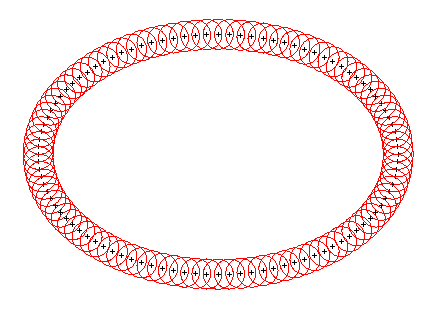
\includegraphics[scale=0.3]{2d/ellipse-balls-15}
    \subcaption{Minkowski sum of an ellipse and balls of radius $ 15 $}

    \includegraphics[scale=0.4]{2d/area/ellipse-100-01-15}
    \includegraphics[scale=0.4]{2d/area/ellipse-100-01-15-100}
    \subcaption{Area flow of an ellipse: 0 / 100 iterations with a timestep of $ 0.1 $}
    \label{fig:ellipse_area_flow}

    \includegraphics[scale=0.4]{2d/perimeter/ellipse-100-01-15}
    \includegraphics[scale=0.4]{2d/perimeter/ellipse-100-01-15-100}
    \subcaption{Perimeter flow of an ellipse: 0 / 100 iterations with a timestep of $ 0.5 $}
    \label{fig:ellipse_perimeter_flow}
\end{figure}

Next, we add some outliers around the ellipse and observe the effects of the two
flows: see \ref{fig:ellipse_outliers_area_flow} and
\ref{fig:ellipse_outliers_perimeter_flow}.

\begin{figure}[h]
    \centering

    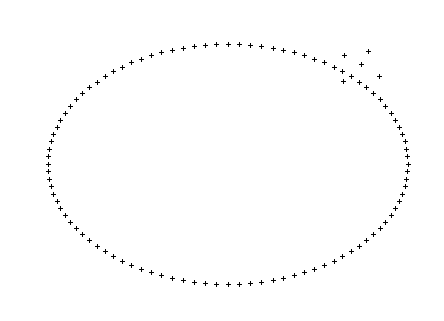
\includegraphics[scale=0.3]{2d/area/ellipse-100-01-15-outliers}
    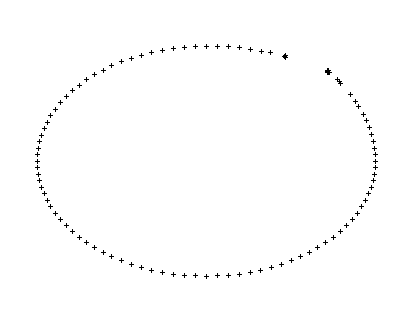
\includegraphics[scale=0.3]{2d/area/ellipse-100-01-15-outliers-40}
    \subcaption{Area flow of an ellipse with outliers: 0 / 40 iterations with a timestep of $ 0.1 $}
    \label{fig:ellipse_outliers_area_flow}

    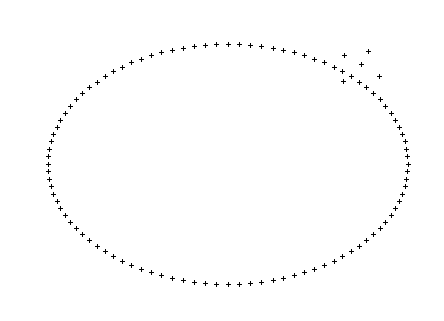
\includegraphics[scale=0.3]{2d/perimeter/ellipse-100-1-15-outliers}
    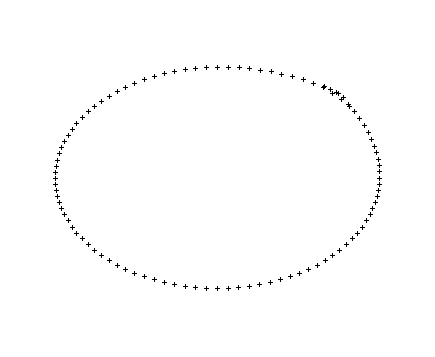
\includegraphics[scale=0.3]{2d/perimeter/ellipse-100-1-15-outliers-100}
    \subcaption{Perimeter flow of an ellipse with outliers: 0 / 100 iterations with a timestep of $ 1 $}
    \label{fig:ellipse_outliers_perimeter_flow}
\end{figure}

Then, we added some Gaussian noise on these points to test the robustness of our
algorithm, see \ref{fig:ellipse_noise_area_flow} and
\ref{fig:ellipse_noise_perimeter_flow}.

\begin{figure}[h]
    \centering

    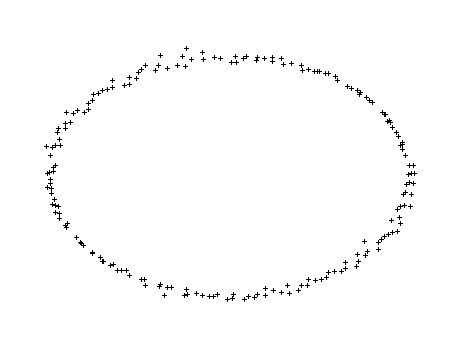
\includegraphics[scale=0.3]{2d/ellipse-noise-5-0}
    \includegraphics[scale=0.3]{2d/area/ellipse-noise-5-75}
    \subcaption{Area flow on a noised ellipse: 0 / 75 iterations with a timestep of $ 0.05 $}
    \label{fig:ellipse_noise_area_flow}

    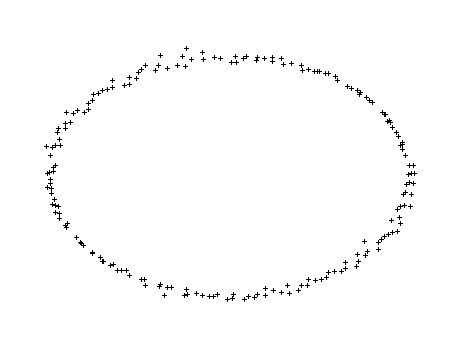
\includegraphics[scale=0.3]{2d/ellipse-noise-5-0}
    \includegraphics[scale=0.3]{2d/perimeter/ellipse-noise-5-75}
    \subcaption{Perimeter flow on a noised ellipse: 0 / 75 iterations with a timestep of $ 0.5 $}
    \label{fig:ellipse_noise_perimeter_flow}
\end{figure}

We notice that the gradient flow of the area may create holes in the point set
which is not the case for the gradient flow of the perimeter.

On the contrary, the gradient flow of the perimeter of the boundary will smooth
the point set while redistributing the points in an uniform way.

% TODO: explain why
This can be explained by looking on a simple case with two intersecting balls:
\begin{itemize}
    \item for the area: TODO
    \item for the perimeter: the gradients are directed towards the outside
        and so the balls will be merged because we can say, using the triangle
        inequality, that in order to minimize the perimeter the balls must come
        closer.
\end{itemize}

The chosen radius will also influence the smoothing: points which are too far
away from other points (at distance greater than the radius) will not move. The
more the radius is big, the more points will move in big groups. Indeed, the
radius indicates how to take the neighbours of a point into account, the more
neighbours we take into account the more "global" the movement will be.

We also tried to add varying oscillations to our ellipse in order to see the
adaptive part of the algorithm. We generate oscillations with one or two
amplitudes.

For one constant amplitude, see \ref{fig:ellipse_osc_perimeter_flow} and
\ref{fig:ellipse_osc_area_flow} and for two different amplitudes see
\ref{fig:ellipse_osc2_area_flow} and \ref{fig:ellipse_osc2_perimeter_flow}.

\begin{figure}[h]
    \centering

    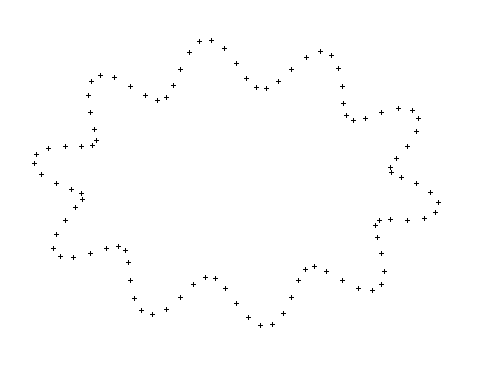
\includegraphics[scale=0.3]{2d/ellipse-osc-25-15-0}
    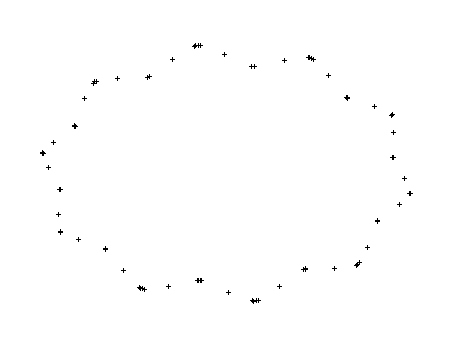
\includegraphics[scale=0.3]{2d/area/ellipse-osc-25-15-25}
    \subcaption{Area flow on an ellipse with oscillations (one amplitude) : 0 /
        25 iterations with a timestep of $ 0.05 $ and a radius of $ 15 $}
    \label{fig:ellipse_osc_area_flow}

    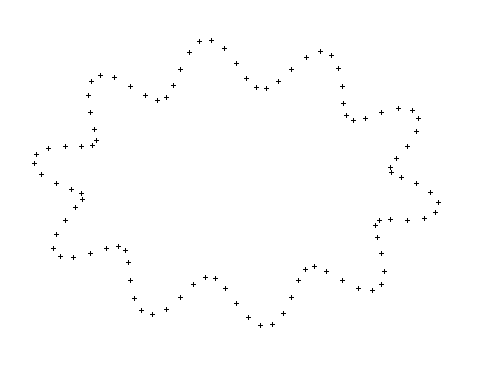
\includegraphics[scale=0.3]{2d/ellipse-osc-25-15-0}
    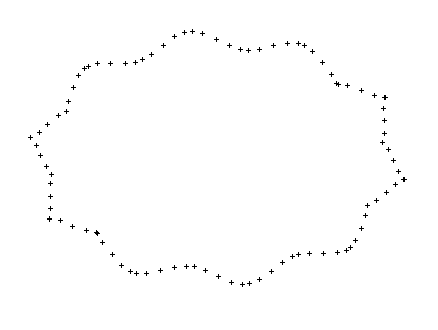
\includegraphics[scale=0.3]{2d/perimeter/ellipse-osc-25-15-50}
    \subcaption{Perimeter flow on an ellipse with oscillations (one amplitude):
        0 / 55 iterations with a timestep of $ 0.5 $ and a radius of $ 15 $}
    \label{fig:ellipse_osc_perimeter_flow}
\end{figure}

\begin{figure}[h]
    \centering

    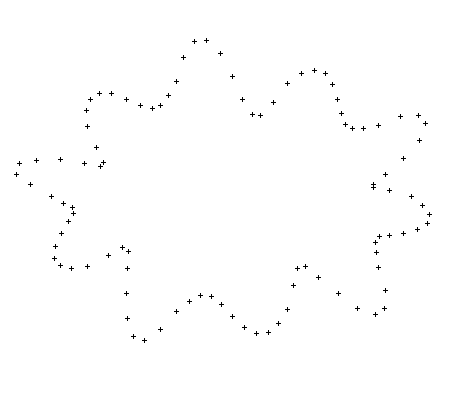
\includegraphics[scale=0.3]{2d/ellipse-osc2-20}
    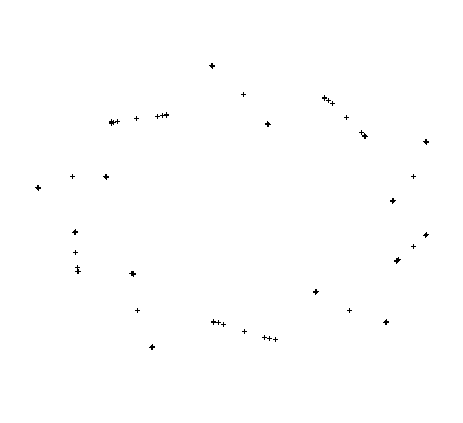
\includegraphics[scale=0.3]{2d/area/ellipse-osc2-20-15-25}
    \subcaption{Area flow on an ellipse with oscillations (two amplitudes): 0 /
        25 iterations with a timestep of $ 0.05 $ and a radius of $ 15 $}
    \label{fig:ellipse_osc2_area_flow}

    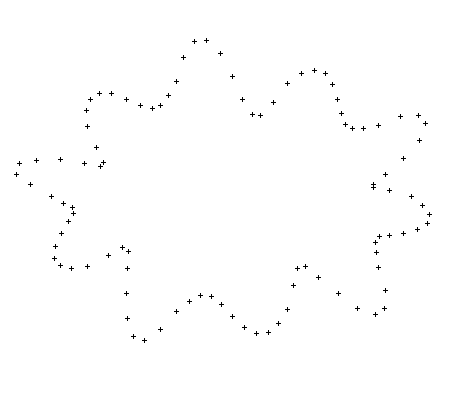
\includegraphics[scale=0.3]{2d/ellipse-osc2-20}
    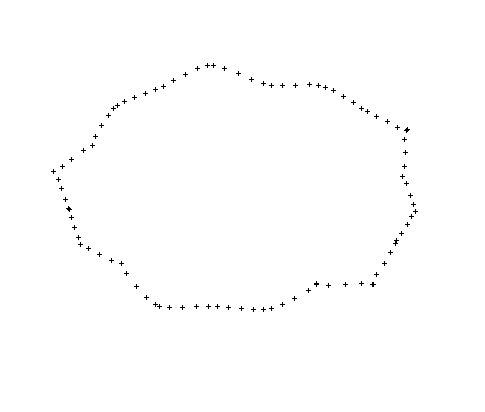
\includegraphics[scale=0.3]{2d/perimeter/ellipse-osc2-20-15-55}
    \subcaption{Perimeter flow on an ellipse with oscillations (two amplitudes)
        : 0 / 55 iterations with a timestep of $ 0.5 $ and a radius of $ 15 $}
    \label{fig:ellipse_osc2_perimeter_flow}
\end{figure}

% TODO: explain why

An other experiment we did is to take points on a line segment and to fix its
endpoints. Then, we apply our flow on this point set. We expect the flow to
smooth the point set: points should get closer and closer to an uniformly
sampled set of points. See \ref{fig:line_fixed_area} and
\ref{fig:line_fixed_perimeter} for the results.

\begin{figure}[h]
    \centering

    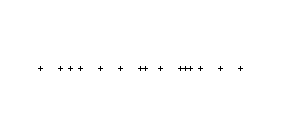
\includegraphics[scale=0.5]{2d/area/line-01-15-0}
    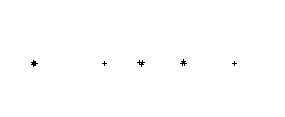
\includegraphics[scale=0.5]{2d/area/line-01-15-50}
    \subcaption{Area flow of points on a segment: 0 / 50 iterations with a timestep of $ 0.1 $}
    \label{fig:line_fixed_area}

    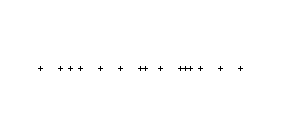
\includegraphics[scale=0.5]{2d/perimeter/line-05-15-0}
    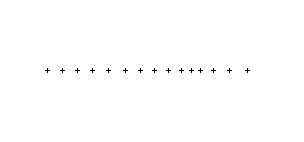
\includegraphics[scale=0.5]{2d/perimeter/line-05-15-50}
    \subcaption{Perimeter flow of points on a segment: 0 / 50 iterations with a timestep of $ 0.5 $}
    \label{fig:line_fixed_perimeter}
\end{figure}

% TODO: explain why

% {{{1 ASSESSMENT
\section{Assessment}

In this chapter, we saw how to simulate discrete mean curvature flows by using
the gradient of the volume of the $r$-offset of a point cloud.

The methods used in this chapter are hard to extend in 3D (see
\cite{cazals2011computing}).

Also, we want to use polyhedral (anisotropic) norms, thing that the previous
method does not allow.

% TODO:
% - description
% - résultats
% - bilan + transition

% vim: set spelllang=en :
